\section{Human-Robot Interaction}
\label{sec:hri}

\subsection{Graphics User Interface}
\label{subsec:gui}
As a domestic service robot, comfortable GUI interaction is neccesary. 
One of the advantage of Pepper is that it has a laptop on its breast, which makes GUI possible. 
We designed a user-friendly and cross-platform interface so even people unfamiliar to robotics can quickly operate on Pepper. 
All applications implemented are integrated in this GUI.

\begin{figure}[h!]

    \centering
    \subfigure[$gui1\_1$]{\label{figa}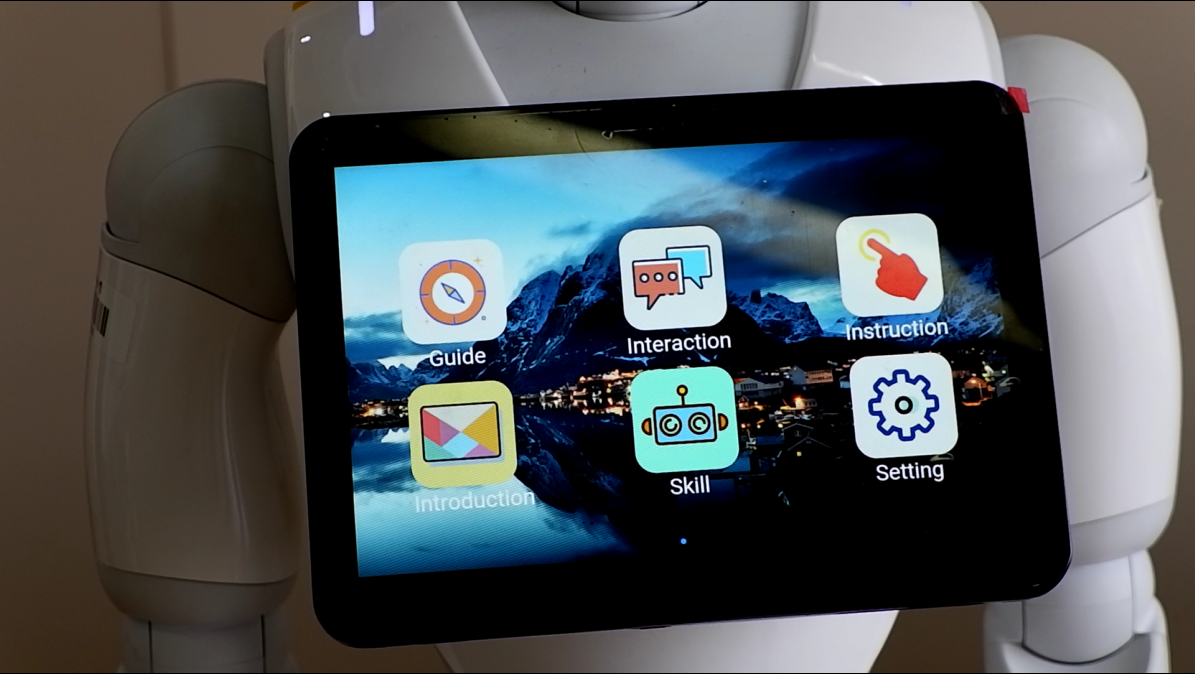
\includegraphics[width=2.5in]{figs/gui1_1.png}}
    \hspace{0.2in}
    \subfigure[$gui1\_2$]{\label{fig:subfig:b}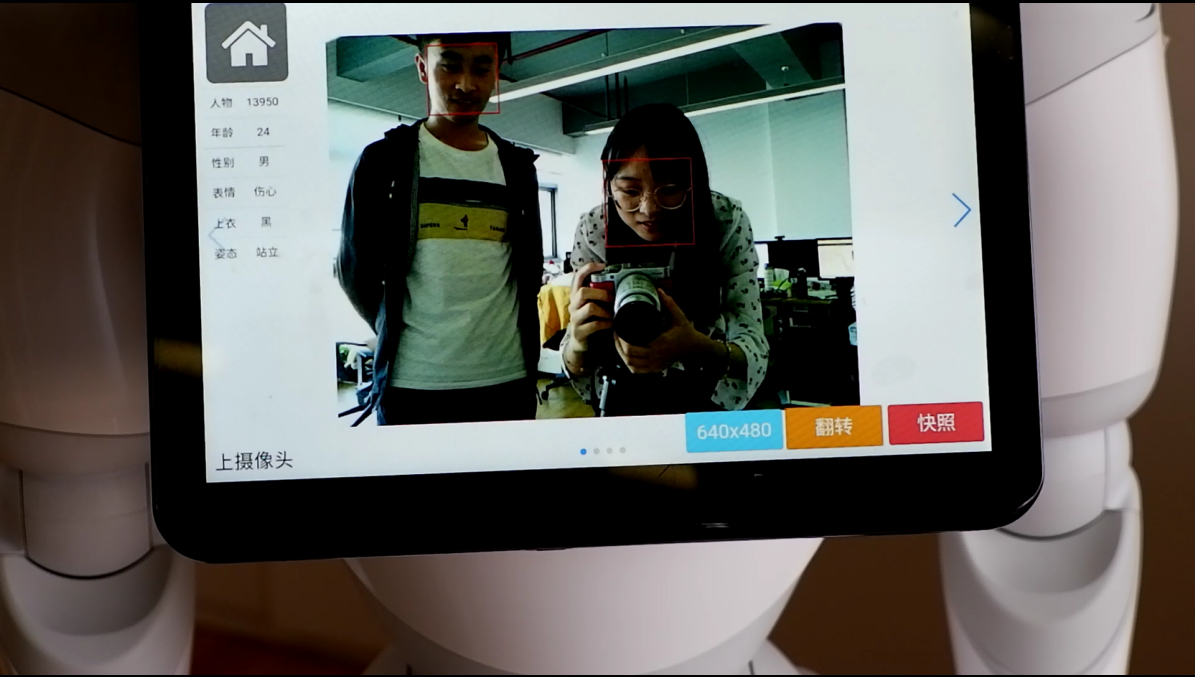
\includegraphics[width=2.5in]{figs/gui1_2.png}}\\
    
    \subfigure[$gui1\_3$]{\label{figa}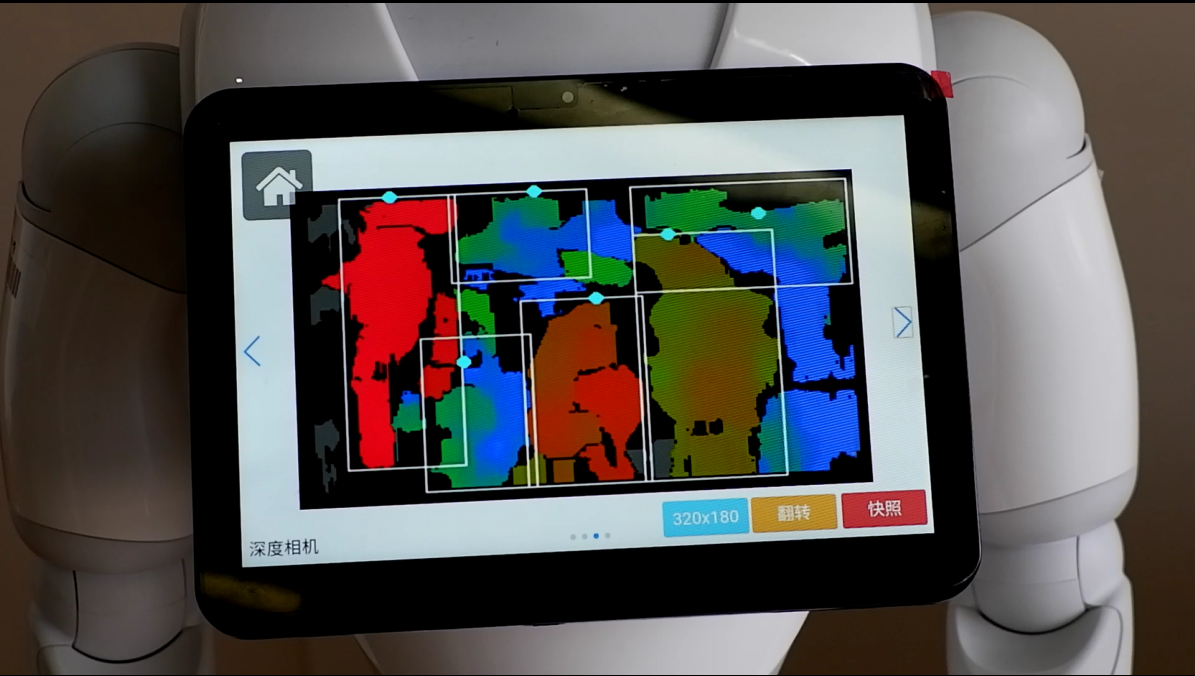
\includegraphics[width=2.5in]{figs/gui1_3.png}}
    \hspace{0.2in}
    \subfigure[$gui1\_4$]{\label{fig:subfig:b}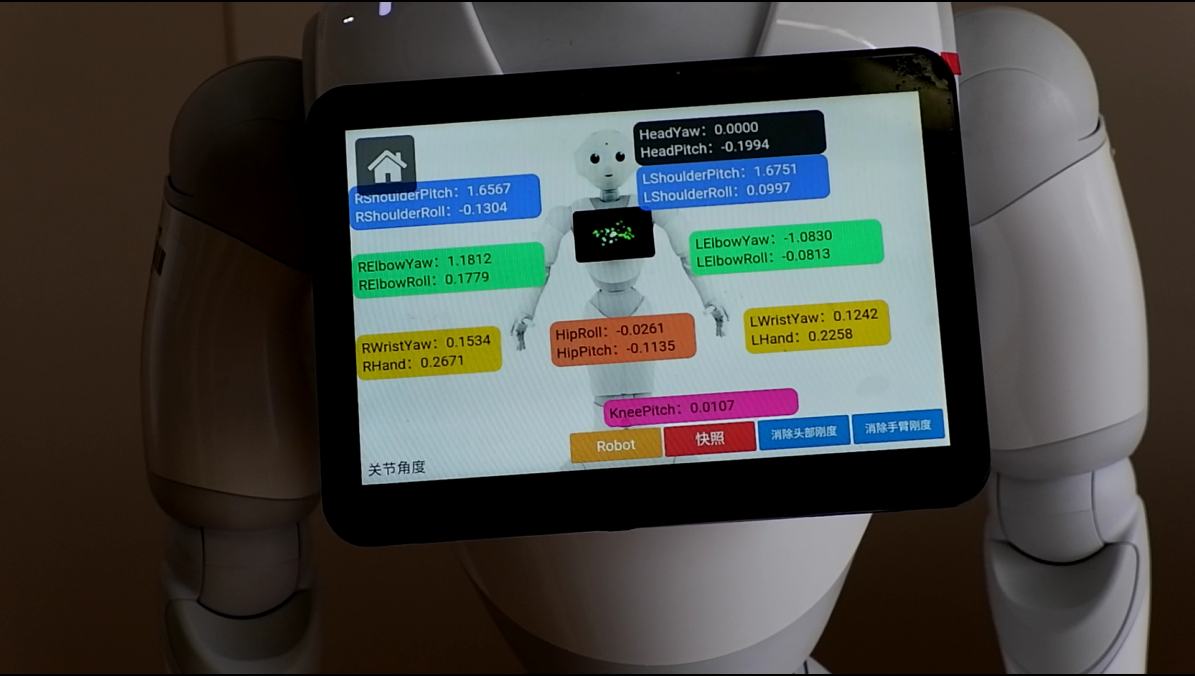
\includegraphics[width=2.5in]{figs/gui1_4.png}}

    \subfigure[$gui1\_5$]{\label{figa}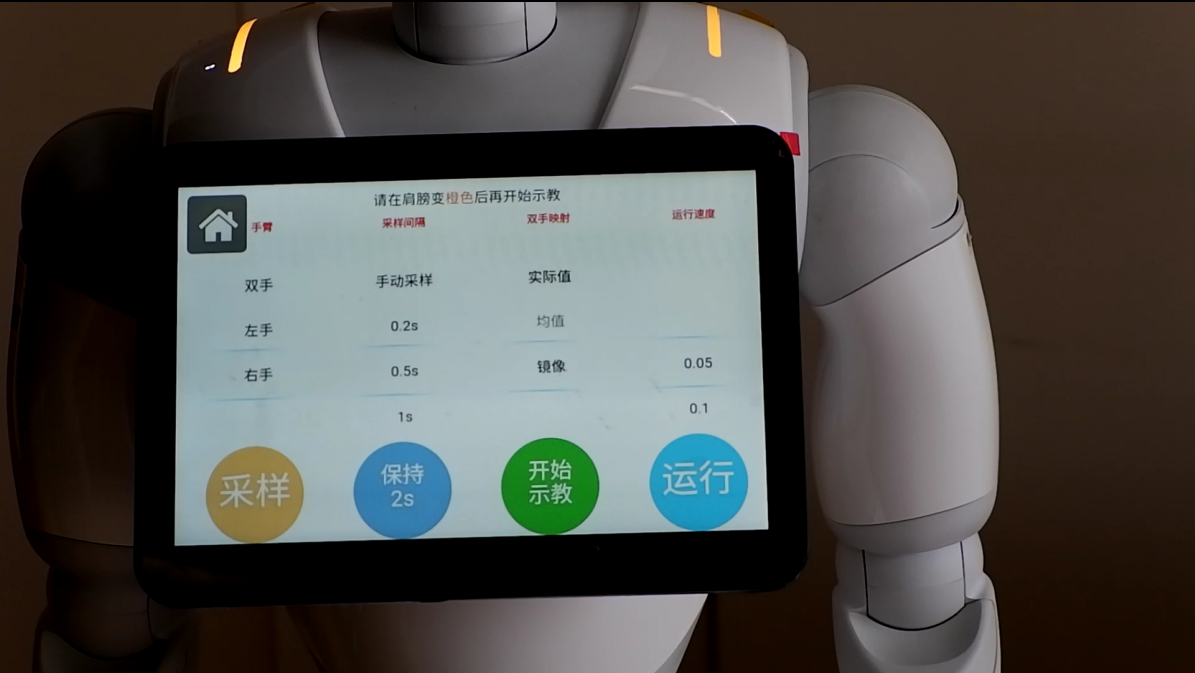
\includegraphics[width=2.5in]{figs/gui1_5.png}}
    \hspace{0.2in}
    \subfigure[$gui1\_6$]{\label{fig:subfig:b}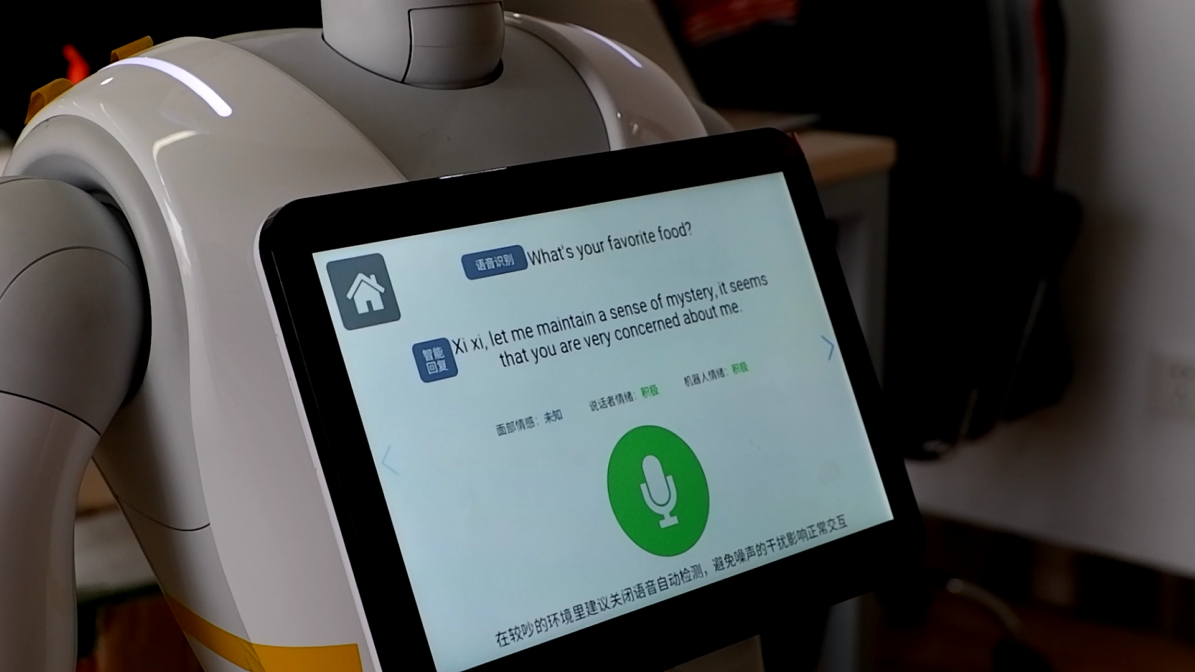
\includegraphics[width=2.5in]{figs/gui1_6.png}}


    \caption{asdjfhskjdhf}
    
    \label{figb} %% label for entire figure
    
    \end{figure}
